\chapter{Introduction}
\label{chap:intro}

\blfootnote{Part of this chapter is adapted from a review in \italicize{Circulation Research} \citep{snellings2021}}
\clearpage



\section{Overview and Significance}
The growth and remodeling of blood vessels is a tightly regulated process that must be maintained from early embryogenesis until death. When this process goes awry blood vessels can become malformed leading to altered, and sometimes pathological function. These malformed blood vessels are termed `vascular malformations' (VMs). VMs may occur anywhere throughout the body, but virtually always occur as focal lesions---affecting one region of the vasculature, rather than presenting as a systemic vascular defect. Even though VMs are focally restricted, they are a source of significant morbidity and mortality in affected individuals. The clinical phenotypes produced by VMs vary substantially, though they are generally prone to rupture (due to increased flow through a fragile vascular bed) or hemorrhage (due to leaky endothelial junctions). The VMs that I will discuss in the following chapters commonly form in the brain and may cause a range of neurological phenotypes including: stroke, epilepsy, seizures, and neurological deficit.

Understanding molecular pathogenesis of VMs is critical for developing methods of treatment and prevention. Although VMs exhibit massive phenotypic heterogeneity, it is becoming increasingly clear that many---if not all---VMs form as a result of somatic mutations.

Somatic mutations are well established as a critical, initiating factor in VM development; however, there remain many types of VM for which the genetic etiology is poorly understood. My dissertation seeks to understand the contribution of somatic mutations to the genetic etiology of Hereditary Hemorrhagic Telangiectasia. Furthermore, I seek to identify novel mechanisms by which somatic mutations fuel the initiation, progression, and predisposition to Cerebral Cavernous Malformations. 

In Chapter 2, I determine that VMs associated with Hereditary Hemorrhagic Telangiectasia (HHT) form via a genetic two-hit mechanism whereby a somatic mutation in \italicize{ENG} or \italicize{ACVRL1} results in biallelic loss of function. HHT is a mendelian disorder inherited by an autosomal dominant allele containing a mutation either \italicize{ENG}, \italicize{ACVRL1}, or \italicize{SMAD4}. Previous studies established that these inherited mutations result in loss of function. This finding lead to the predominant theory that the VMs associated with HHT are the result of haploinsufficiency. However, this theory is inconsistent with the presentation of VMs in HHT. The VMs associated with HHT present as focal lesions, rather than manifesting as a systemic vascular defect as might be expected by haploinsufficiency. This disconnect suggests that a local event is necessary for the development of VMs in HHT. I tested whether this local event may be a somatic mutation in the single remaining wild-type allele of the mutated gene. Such a mutation would cause in biallelic loss of function and result in the complete loss of functional gene product in the cells harboring the somatic mutation. I sequenced 19 telangiectasia (a cutaneous VM) from individuals with HHT and found a loss of function somatic mutation in 9 of 19 telangiectasia. Each somatic mutation I identified occurred in the same gene as the respective inherited mutation. Using long-read sequencing I showed that pairs of somatic and germline mutations exist in a \italicize{trans} configuration, confirming that these mutations resulted in biallelic loss of function. Furthermore I showed that multiple telangiectasia from the same individual harbored unique somatic mutations, suggesting that each telangiectasia is initiated by a different mutational event rather than a metastasis-like mechanism. 

In Chapter 3, I identify a novel somatic mutation in Cerebral Cavernous Malformations (CCMs) that occurs in the \italicize{same cell} as additional somatic mutations that synergize to fuel CCM progression. Similar to HHT, CCM is a mendelian disorder inherited by an autosomal dominant allele containing a mutation in either \italicize{KRIT1}, \italicize{CCM2}, or \italicize{PDCD10}. Previous studies established that CCMs are caused by somatic mutations via a genetic two-hit mechanism similar to what I describe in Chapter 2. The two-hit mechanism tidily explains the variable penetrance of the inherited disorder and explains why sporadic cases have a single CCM whereas inherited cases have many; however, the two-hit mechanism does not account for the extreme variation in the severity of CCMs in the same individual, nor why some CCMs rapidly grow after years of quiescence. I hypothesized that some of the most aggressive CCMs may harbor somatic mutations in other genes that fuel CCM growth. To test this hypothesis, I sequenced 79 sporadic and inherited CCMs and found that 71\% of these CCMs all had a gain of function somatic mutation in the same gene: \italicize{PIK3CA}. Surprisingly, many of the CCMs had mutations in \italicize{PIK3CA} \italicize{and} either \italicize{KRIT1}, \italicize{CCM2}, or \italicize{PDCD10}; as many as three distinct somatic mutations within a single lesion. This finding prompted a new question: are all of the mutations present within the same cell, or are two different populations of cells merging to form a mosaic CCM? To answer this question, I collected nuclei from frozen CCM samples and sequenced the DNA from individual nuclei to determine the cellular phase of the somatic mutations. I sequenced a total of 21,221 nuclei across 2 inherited and 6 sporadic CCMs and all 8 confirmed that the somatic mutations are present within a single clonal population of cells. This study is the first to find that multiple genes contribute to the pathogenesis of a vascular malformation and highlights \italicize{PIK3CA} as a major contributor to CCM progression. In addition, the identification of \italicize{PIK3CA} mutations suggested rapamycin (an inhibitor of PI3K signaling) as a potential therapeutic for CCM and has since proved highly effective in preventing CCMs in mice. 

In Chapter 4, I find that Developmental Venous Anomalies (DVA) are caused by a somatic mutation in \italicize{PIK3CA} and predisposes to the formation of CCMs. The finding in Chapter 3 that some CCMs harbor as many as three distinct somatic mutations all within the same cell was somewhat surprising. Multiple mutations are common in cancer, but cancer develops in the context of uncontrolled growth and genomic instability. To understand how multiple mutations were occurring in CCMs we looked for signs of genomic instability in CCMs via sequencing and stains for DNA damage but found no evidence of elevated mutation rates. Instead, I found an answer in the form of DVA. DVA are the most common vascular malformation, present in up to 16\% of the population. DVA are considered to be harmless; however, almost all sporadic CCM form directly adjacent to a DVA. The association of DVA and CCM has been known for decades, but the cause has remained a mystery. I hypothesized that DVA could result from somatic \italicize{PIK3CA} mutation during developmental angiogenesis, creating a field of mutant cells that may develop into a CCM upon subsequent mutations. I tested this hypothesis using droplet digital PCR and found that \italicize{PIK3CA} mutation was present in both the CCM and the associated DVA, but that other pathogenic somatic mutations were found exclusively in the CCM. These data suggest that DVA are acting as a genetic primer that predisposes to CCM formation.

My results demonstrate that somatic mutations play an integral role in the development of VMs associated with HHT and CCM, and constitutes the first evidence of a VM that develops as a result of digenic somatic mutations. This opens new avenues of research into the mechanisms VM development, and identifies promising therapeutics that are currently being pursued for clinical trials. Before describing my results in detail, the remainder of this chapter provides a brief introduction to vascular malformations and previous research into HHT and CCM.



\section{Background}
Vascular malformation is a general term that encompasses a wide breadth of vascular phenotypes ranging from simple birthmarks to disfiguring, and life-threatening lesions. Despite these differences, vascular malformations share several important properties that are useful to examine in the context of their counterpart: vascular tumors. Vascular tumors, like other types of tumors, are characterized by rapid and uncontrolled growth. In contrast, vascular malformations typically do not grow uncontrollably but rather tend to grow proportionally to the individual. There are of course exceptions of vascular malformations that grow rapidly, which will be a focus of Chapter 3. In addition, vascular malformations are generally more stable than vascular tumors. Vascular tumors have a prominent growth phase which is often is followed by spontaneous involution resulting in complete regression of the lesion. This is especially true of infantile hemangiomas, the most common type of vascular tumor which I will briefly discuss in Chapter 5. In contrast, the spontaneous regression of vascular malformations is very rare.

Vascular malformations are further divided by the type of vascular bed affected: arteries, veins, capillaries, or lymphatic vessels. While a vascular malformation may be restricted to a single type of vessel, they are often observed as mixed vascular malformations (e.g.~arterio-venous malformation) and mixed vascular-lymphatic malformations (e.g.~capillary-lymphatic-venous malformation). Vascular malformations are also identified by the rate of flow through the lesion, namely low-flow and high-flow. The rate of flow is generally a function of the type of vascular bed affected; with arterial and mixed-arterial malformations generally being high-flow; and venous, capillary, lymphatic malformations being low-flow. The rate of flow is a useful identifier as it helps inform the type of complications the individual may encounter: high-flow lesions are prone to rupture, whereas low-flow lesions prone to hemorrhage.

While many vascular malformations form sporadically, they may also occur in association with an inherited disorder. The chapters that follow focus on two such disorders: Hereditary Hemorrhagic Telangiectasia, and Cerebral Cavernous Malformations. 



\subsection{Hereditary Hemorrhagic Telangiectasia}
Hereditary Hemorrhagic Telangiectasia (HHT) is a genetic disease characterized by abnormal direct connections between arteries and veins resulting in high-flow lesions called arteriovenous malformations (AVMs). Individuals with HHT often have small AVMs called telangiectasia on mucosal (GI, lips, tongue, inner eyelids) and dermal (face, fingers, nail beds) surfaces (Figure~\ref{HHT_AVM}A). In addition, some individuals with HHT develop pulmonary (Figure~\ref{HHT_AVM}B), hepatic, and brain AVMs (Figure~\ref{HHT_AVM}C). These visceral AVMs are typically larger and carry considerably more risk compared to telangiectasia. 

%%%%%%%%%%%%%%%%%%%%%%%%%%%%%%
%				     FIGURE 1					%
%%%%%%%%%%%%%%%%%%%%%%%%%%%%%%
\begin{figure}[bp!]
\begin{center}
\includegraphics[width=5in]{HHT_AVM}
\end{center}
\caption[Vascular Malformations in HHT.] {\textbf{Vascular Malformations in HHT.} \\ \textbf{A}, Telangiectasia on the lip of an individual with HHT. Case courtesy of Herbert L. Fred and Hendrik A. van Dijk. \textbf{B}, 3D render of a CT scan showing a pulmonary AVM creating a shunt between a pulmonary arterial branch and a pulmonary vein tributary (arrow). Case courtesy of Vikas Shah. \textbf{C}, The cross section of a large brain AVM in the right hemisphere.}

\label{HHT_AVM}
\end{figure}
%%%%%%%%%%%%%%%%%%%%%%%%%%%%%%

\subsubsection{Genetics}
HHT is an autosomal dominant disease known to be caused by mutations in one of three causal genes: \italicize{ENG} \citep{mcallister1994}, \italicize{ACVRL1} \citep{johnson1996}, and \italicize{SMAD4} \citep{gallione2004}. Mutations in \italicize{ENG} and \italicize{ACVRL1} account for roughly 85\% of HHT cases, though as high as 96\% has been reported when the Cura\c{c}ao criteria are strictly followed \citep{mcdonald2020}. Mutations in \italicize{SMAD4} cause the combined disorder of juvenile polyposis and HHT (JP-HHT); these mutations account for only 2\% of HHT cases. Mutations that cause HHT are known to result in the loss of function of the affected gene. In \italicize{ENG} roughly 80\% of pathogenic mutations result in premature termination either through frameshift or nonsense mutations. In contrast, 53\% of pathogenic mutations in \italicize{ACVRL1} are missense changes, the majority of which occur in modest hotspots throughout the intracellular kinase domain \citep{abdalla2003}. This difference may be attributed to the relative intolerance of missense changes in \italicize{ACVRL1} compared to \italicize{ENG} as shown by the low number of common missense variants in the gnomad database (\italicize{ENG}: expected 389.9, observed 338; \italicize{ACVRL1}: expected 311.5, observed 190) Compared to the other genes, \italicize{ACVRL1} also has a high number of splice variants, including a 300bp CT-rich region in intron 9 \citep{wooderchakdonahue2018}. In \italicize{SMAD4}, mutations causing JP-HHT are a mix of missense and nonsense/frameshift; the vast majority of which are found in exons 8--11, overlapping the MH2 domain of SMAD4 \citep{gallione2004}.

There remain a minority of individuals who fulfill all of the clinical diagnostic criteria of HHT (the Cura\c{c}ao criteria) yet sequencing and CNV analysis reveal no pathogenic mutation in \italicize{ENG}, \italicize{ACVRL1}, or \italicize{SMAD4}. In these cases, one possibility is that a pathogenic mutation does exist in one of these genes, however it is labeled as variant of unknown significance, or the mutation occurs in regions not covered by the sequencing panel (i.e. variants in introns or promoter regions). One other alternative is that mutations in other unidentified genes may cause HHT. In the past there have been some indications that genes besides \italicize{ENG}, \italicize{ACVRL1}, and \italicize{SMAD4} may cause HHT. In 2005 and 2006 two new loci linked to HHT were mapped to chromosome 5 and 7 respectively \citep{cole2005, bayraktoydemir2006}. Despite this finding, no additional cases have been identified mapping to these regions, nor have any causal genes been identified. Recent work has identified the gene \italicize{GDF2} which encodes the protein BMP9 as a potential causal gene for HHT \citep{wooderchakdonahue2013}. There are currently two published reports of \italicize{GDF2} variants in individuals with HHT-like phenotypes found by sequencing samples sent for HHT diagnostic testing, but with no identified mutation in the known causal genes \citep{wooderchakdonahue2013, hernandez2015}. Combining these studies, a total of 5 individuals with HHT-like phenotypes have been reported with five different \italicize{GDF2} variants. However, two of the 5 variants (c.997C$>$T and c.-51C$>$A) are present in the general population with frequency higher than HHT (HHT: $1\times 10^{-4}$; variant gnomAD v2 population frequencies: 4.07$\times 10^{-4}$, and 2.48$\times 10^{-4}$ respectively). A third variant, c.950G$>$A is present in the general population at 0.44$\times$ the frequency of HHT (4.38$\times 10^{-5}$). These data suggest that these three variants do not cause HHT. The remaining two variants (c.254C$>$T, c.203G$>$T) are extremely rare in the general population and may potentially be pathogenic. Specifically, c.203G$>$T has been found to segregate in a family with 3 individuals with epistaxis. Despite this evidence, the rarity of these mutations, and the incomplete phenotypic overlap with HHT suggests that if these variants are indeed pathogenic, they cause a rare vascular disease overlapping with HHT but should not be considered an HHT causal gene, though \italicize{GDF2} would be an appropriate addition to vascular anomaly diagnostic sequencing panels. 

\subsubsection{Animal Models}
Our understanding of the genetics of HHT has led to the development of mouse models that recapitulate the disease phenotype. The first mice created were made with heterozygous germline loss of either \italicize{Eng} or \italicize{Acvrl1} (\italicize{Eng}$^{+/-}$ and \italicize{Acvrl1}$^{+/-}$ respectively). These heterozygous mice match the genotype of humans with HHT, however these mice have a very mild phenotype that only presents in a small fraction of mice \citep{bourdeau1999, torsney2003, srinivasan2003}. As the heterozygous mice did not produce a robust and reproducible phenotype, we wished to create a more aggressive model via homozygous knockout mice: \italicize{Eng}$^{-/-}$ and \italicize{Acvrl1}$^{-/-}$. However, this was challenging as germline homozygous loss of these genes results in embryonic lethality due to vascular defects \citep{li1999, bourdeau1999, oh2000, arthur2000}. To circumvent the embryonic lethality, we generated mice where gene deletion could be induced by injecting the mice with tamoxifen using the Cre-Lox system \citep{allinson2007, park2008}. These homozygous inducible mice allowed us to delete both alleles of \italicize{Eng} or \italicize{Acvrl1} postnatally and circumvent embryonic lethality. Surprisingly, inducing gene deletion after developmental angiogenesis had almost no affect on the vasculature. However, several groups found that pairing induced gene deletion while also stimulating vascular growth (e.g. wound healing, VEGF) resulted in robust and reproducible AVM formation \citep{park2008, walker2011, choi2012, chen2013}.

\subsubsection{Sporadic Brain AVMs}
While AVMs are common in individuals with HHT, the majority of all AVMs are sporadic, occuring in unrelated individuals with no known genetic predisposition. These sporadic AVMs disproportionally occur in the brain. Molecular studies of sporadic brain AVMs has found that the majority harbor a somatic activating mutation in \italicize{KRAS}, a commonly mutated oncogene \citep{nikolaev2018}. Studies comparing the severity of sporadic and HHT-associated AVMs are sparse, however I have discussed this topic with several surgeons who operate on AVMs and the consensus is that sporadic AVMs tend to be larger and more aggressive than HHT-associated AVMs. This observation may suggest that sporadic and HHT-associated AVMs develop via different genetic mechanisms. HHT-associated AVMs are rarely surgically resected (in favor of embolism) therefore it has been challenging to assess the presence of \italicize{KRAS} mutations in HHT-associated AVMs; however, given the clear heredity of brain AVMs in HHT, it is unlikely that HHT-associated AVMs develop from a somatic \italicize{KRAS} mutation. 



\subsection{Cerebral Cavernous Malformation}
Cerebral Cavernous Malformation (CCM) is a genetic disease characterized by the formation of the eponymous vascular malformations---CCMs---in the brain and spinal cord. CCMs form in the capillaries that connect arteries and veins, specifically in postcapillary venules. CCMs consist of multiple `caverns' that fill with blood resulting in a slow-flow vascular malformation similar in appearance to a raspberry. Similar to AVMs, CCMs may form as a result of the familial disease, or sporadically in otherwise healthy individuals. Those with familial CCM typically develop numerous CCMs (Figure~\ref{CCM_Lesion}A) whereas sporadic cases of CCM almost always present as a single solitary lesion (Figure~\ref{CCM_Lesion}B). 

%%%%%%%%%%%%%%%%%%%%%%%%%%%%%%
%				     FIGURE 2					%
%%%%%%%%%%%%%%%%%%%%%%%%%%%%%%
\begin{figure}[tbp!]
\begin{center}
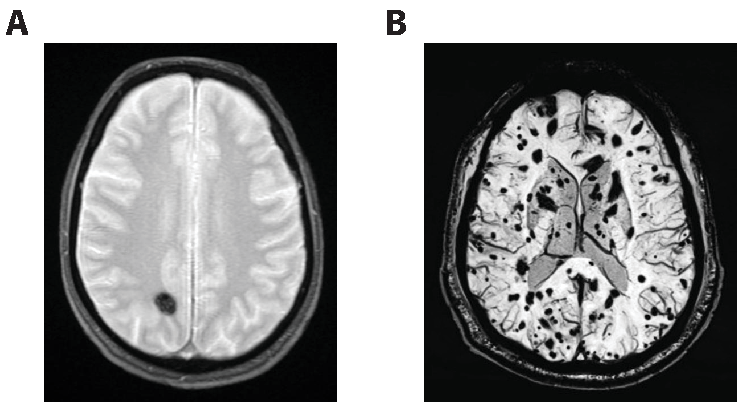
\includegraphics[width=5in]{CCM_Lesion}
\end{center}
\caption[Cerebral Cavernous Malformations.] {\textbf{Cerebral Cavernous Malformations.} \\ \textbf{A},  A sporadic CCM presenting as a solitary lesion in the hindbrain. Case courtesy of Bruno Di Muzio. \textbf{B}, The brain of an individual with familial CCM presenting with numerous lesions throughout their brain. Case courtesy of Frank Gaillard.}

\label{CCM_Lesion}
\end{figure}
%%%%%%%%%%%%%%%%%%%%%%%%%%%%%%

\subsubsection{Developmental Venous Anomalies}
Although sporadic CCMs form in individuals with no known genetic predisposition, sporadic CCMs are known to be closely associated with developmental venous anomalies (DVA). DVA are the single most common vascular malformations affecting up to 16\% of people \citep{brinjikji2017}, and are often found to directly abut a sporadic CCM. Several studies have reported that 24--32\% of sporadic CCMs abut a DVA based on MR imaging \citep{abdulrauf1999, wurm2005, porter1999}; however, in surgically resected CCM lesions, Porter et al. identified an intimately associated DVA in every of 86 resected lesions \citep{porter1999}. In addition, several groups have reported that use of more powerful imaging techniques reveal DVA associated with CCM lesions that were otherwise missed with standard MR imaging \citep{dammann2017, kamezawa2005}---suggesting the frequency of associated DVA and CCM is underestimated. Despite the common association between sporadic CCM and DVA, DVA are rarely ever found in association with familial CCM \citep{petersen2010}, suggesting that DVA have a yet unknown role in the pathogenesis of specifically sporadic---but not familial---CCM.

%%%%%%%%%%%%%%%%%%%%%%%%%%%%%%
%				     FIGURE 3					%
%%%%%%%%%%%%%%%%%%%%%%%%%%%%%%
\begin{figure}[tbp!]
\begin{center}
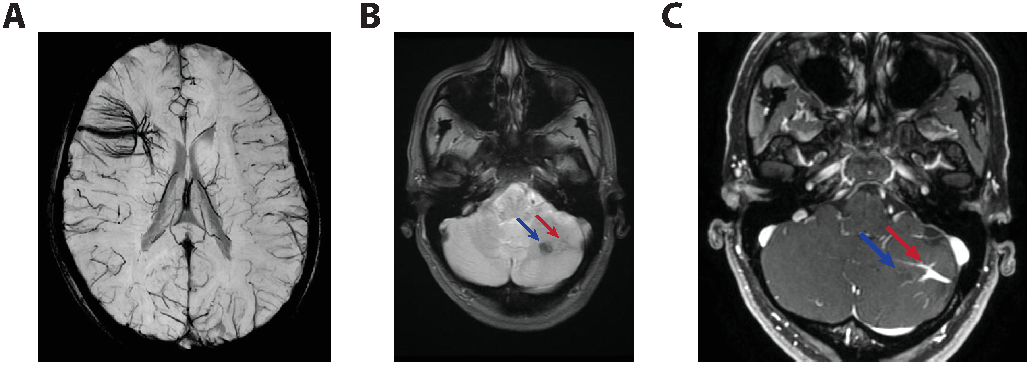
\includegraphics[width=5.8in]{DVA_Lesion}
\end{center}
\caption[Developmental Venous Anomalies.] {\textbf{Developmental Venous Anomalies.} \\ \textbf{A},  A DVA with a characteristic caput medusae (palm tree-like appearance) in the left hemisphere. Case courtesy of Neil Lall. \textbf{B--C}, MR imaging of one case of an associated DVA and CCM visualized with either an Axial Gradient Echo (B) or an Axial T1 C+ (C). The Axial Gradient Echo shows the CCM best (blue arrow), whereas the Axial T1 C+ shows the DVA best (red arrow)}

\label{DVA_Lesion}
\end{figure}
%%%%%%%%%%%%%%%%%%%%%%%%%%%%%%

\subsubsection{Germline Genetics}
Familial CCM follows an autosomal dominant pattern of inheritance \citep{bicknell1978, clark1970, kidd1947} and is caused by heterozygous loss of function (LOF) mutations in either \italicize{KRIT1} \citep{labergelecouteulx1999, sahoo1999}, \italicize{CCM2} \citep{liquori2003, denier2004}, or \italicize{PDCD10} \citep{bergametti2005}. The protein products of these genes bind to each other to form the `CCM Complex' which is involved in signal transduction related to vascular development. Mutations in these genes primarily consist of nonsense, frameshift, and canonical splice site mutations. Pathogenic missense mutations have been reported in all three genes; however, they make up the minority of reported mutations. Notably, there are 4 known founder mutations in the CCM genes that account for substantial fraction of familial CCM cases. The most common of these is NM\_194456.1(\italicize{KRIT1}):c.1363C$>$T(p.Gln455Ter) present in most Hispanic American cases of familial CCM \citep{gunel1996, sahoo1999}. Another less frequent \italicize{KRIT1} founder mutation: NM\_194456.1(\italicize{KRIT1}):c.987C$>$A(p.Cys329Ter), has been found in several kindreds with Sardinian lineage \citep{cau2009}. A deletion spanning 77.6kb of \italicize{CCM2} resulting in deletion of exons 2--10 has been found in several Caucasian kindreds, it remains unclear whether all cases with this mutation are related or whether it has occurred independently in other families \citep{liquori2007}. A splice mutation affecting \italicize{CCM2}: NM\_031443.3(\italicize{CCM2}):c.30+5\_30+6delinsTT, has been found in seemingly unrelated Ashkenazi Jewish probands, possibly due to an historically ancient mutation \citep{gallione2011}.

\subsubsection{Genotype-Phenotype Correlation}
The clinical manifestations of familial CCM are highly heterogeneous. In many genetic diseases, the primary determinant of progression and severity is the causal mutation. However, this does not seem to be the case for CCM. A prime example of this is the common Hispanic founder mutation. Disease progression and severity in individuals with the Hispanic founder mutation is highly variable, despite sharing an identical pathogenic mutation \citep{gault2006, laurans2003, denier2004, gianfrancesco2007}. The lack of correlation between clinical manifestations and mutation identity is consistent with the finding that the majority of germline mutations found in \italicize{KRIT1}, \italicize{CCM2}, and \italicize{PDCD10}---primarily frameshift, nonsense, and splice site mutations---result in loss of function. This suggests that the identity of mutations within the same gene does not have a significant impact on disease severity.

Though different mutations within a gene do not seem to impact disease severity, the identity of the mutated gene has been associated with several clinical characteristics. Many groups have noted an association between individuals with \italicize{KRIT1} mutations and cutaneous vascular lesions \citep{gianfrancesco2007, sirvente2009, musunuru2003, grippaudo2013, wang2013, eerola2000, labauge1999}. Individuals with a mutation in \italicize{CCM2} are more likely to be asymptomatic and have lower number of lesions compared to individuals with \italicize{KRIT1} or \italicize{PDCD10} mutations \citep{denier2006}. Familial CCM is significantly more aggressive in individuals with a mutation in \italicize{PDCD10} \citep{fauth2015, shenkar2015, riant2013}. The severity of CCM associated with \italicize{PDCD10} mutations is attributable to the role of \italicize{PDCD10} in the gut epithelium not shared with \italicize{KRIT1} or \italicize{CCM2} \citep{tang2019}. 

\subsubsection{Genetic Modifiers}
To identify genetic variants associated with disease severity, one group performed a large genetic association study of individuals with the \italicize{KRIT1} founder mutation that identified several genetic polymorphisms within inflammatory and immune response genes that are associated with total lesion count, number of large lesions, and intracerebral hemorrhage \citep{choquet2014}. This analysis revealed associations between clinical disease presentation and variants in several genes including: \italicize{TGFBR2}, \italicize{CD14}, \italicize{IL6R}, \italicize{MSR1}, \italicize{IGH}, and \italicize{TLR4}. Some of these genes have been shown to have critical roles in CCM pathogenesis, highlighting the importance of further evaluating the roles of these genes, and demonstrating the power of association studies in a genetically homogenous cohort. Identification of TLR4 variants associated with disease severity are of particular interest owing to the direct role of \italicize{TLR4} in propagating CCM signaling \citep{tang2019}. These data suggest that polymorphisms in genes other than \italicize{KRIT1}, \italicize{CCM2}, and \italicize{PDCD10} may be important modifiers of CCM pathogenesis. 

\subsubsection{Radiation-Induced CCMs}
While the majority of sporadic CCMs occur in otherwise healthy individuals, numerous reports have shown that ionizing radiation is a potent inducer of CCM formation \citep{cutsforthgregory2015, heckl2002, jain2005, burn2007, strenger2008, vinchon2011, koike2012, martinezlage2008, novelli1997, baumgartner2003}. While pathologically similar to non-radiation induced sporadic CCMs, they have several distinct characteristics that hint at the underlying mechanisms driving CCM pathogenesis. One such characteristic is that individuals with radiation-induced CCMs often present with multiple lesions, in stark contrast to non-radiation induced sporadic CCMs which almost always occur as a solitary lesion. Furthermore, it was found that occurrence of multiple radiation-induced CCMs is significantly associated with younger age at time of radiation treatment \citep{cutsforthgregory2015} and that the presence of multiple radiation induced CCMs may be related to higher doses of ionizing radiation \citep{novelli1997}. Ionizing radiation has long been recognized as a potent source of DNA damage leading to genomic instability reviewed elsewhere \citep{little1998}. The observation that radiation treatment may induce CCM formation---and that the multiplicity of lesions is related to radiation dose and age at radiation---support a key role for somatic mutations in CCM pathogenesis.

\subsubsection{Somatic Mutation Cause CCM Via a Two-Hit Mechanism}
Although germline LOF mutations in \italicize{KRIT1}, \italicize{CCM2}, or \italicize{PDCD10} cause familial CCM as a clinical entity, they do not explain why CCMs present as focal lesions rather than a systemic vascular defect as might be expected if CCMs were the result of haploinsufficiency. This observation led to the hypothesis that a secondary, local event is necessary to initiate lesion formation; specifically, a somatic mutation in a CCM gene resulting in biallelic LOF. Somatic mutations resulting in biallelic LOF of \italicize{KRIT1}, \italicize{CCM2}, or \italicize{PDCD10} have been reported in both familial \citep{gault2005, akers2009, gault2009} and sporadic \citep{mcdonald2014} CCMs. Furthermore, laser capture microdissection and immunohistochemical staining of the CCM proteins in the lesion endothelium has established that these mutations occur in endothelial cells \citep{akers2009, pagenstecher2009, rath2020}. Together these data show that while loss of a CCM gene is dominant at the level of an individual, it is recessive on a cellular level, requiring loss of the normal allele via somatic mutation prior to lesion formation (Figure~\ref{CCM_TwoHitIntro}).   

%%%%%%%%%%%%%%%%%%%%%%%%%%%%%%
%				     FIGURE 4					%
%%%%%%%%%%%%%%%%%%%%%%%%%%%%%%
\begin{figure}[tbp!]
\begin{center}
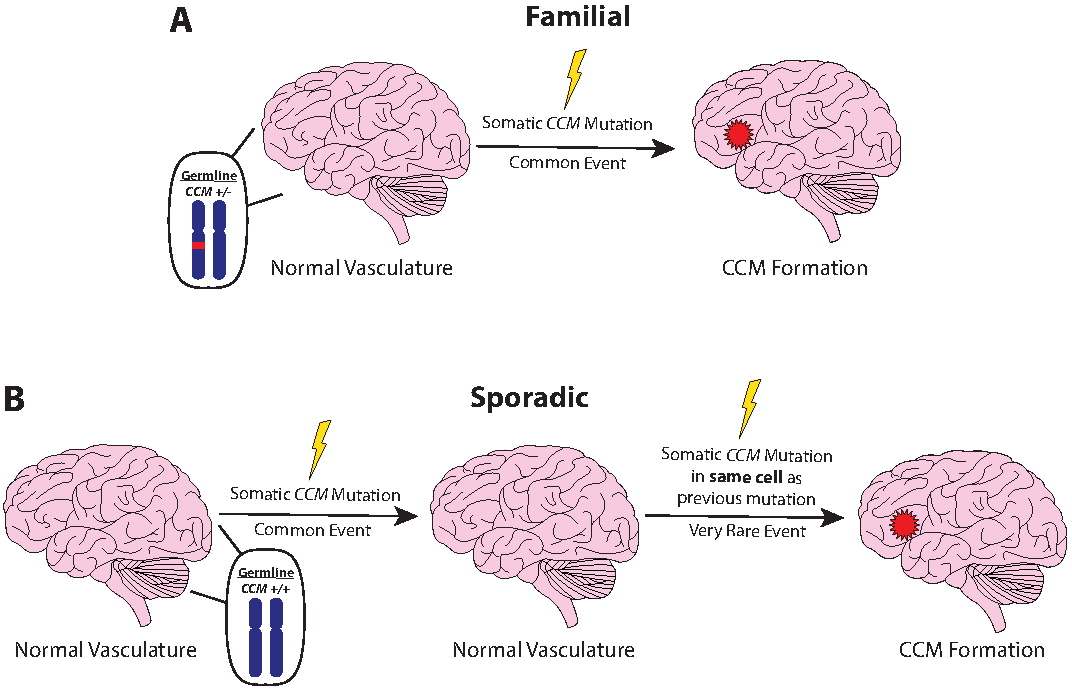
\includegraphics[width=5.8in]{CCM_TwoHitIntro}
\end{center}
\caption[Two-Hit Mechanism of CCM Pathogenesis.] {\textbf{Two-Hit Mechanism of CCM Pathogenesis.} \\ \textbf{A}, Two-Hit model for familial CCM where the starting state is heterozygous and a somatic mutation results in loss of the second allele. \textbf{B}, Two-Hit model for sporadic CCM where the starting state is wild type and two somatic mutations \italicize{in the same cell} are required to initiate lesion formation.}

\label{CCM_TwoHitIntro}
\end{figure}
%%%%%%%%%%%%%%%%%%%%%%%%%%%%%%

\subsubsection{Animal Models}
The two-hit mechanism of CCM pathogenesis has been implemented in mice to generate a phenotype closely resembling the human disease. Inducible homozygous deletion of \italicize{Krit1}, \italicize{Ccm2}, or \italicize{Pdcd10} leads to robust formation of CCMs. However, one limitation of these models is that the capacity to form CCM is highly dependent on the time of gene deletion. If gene deletion occurs on postnatal day 1 (P1), the mice develop numerous large CCMs with strong enrichment in the cerebellum. After P1 the lesion burden steadily decreases and if gene deletion occurs later than P10, the mice do not develop CCMs even when aged \citep{boulday2011, detter2020}. This phenomenon likely reflects a dependence on active angiogenesis for CCM formation in these mice. During development the there is a well-established `angiogenic window' where the vasculature in the brain is actively growing \citep{boulday2009}. Notably, angiogenesis is strongest in the cerebellum in the first few days after birth, which is consistent with the strong enrichment of CCMs in the cerebellum at this timepoint \citep{boulday2009}. This facet of the CCM mouse models is at odds with the human phenotype. While many CCMs are congenital, there are also many cases of CCM development in adulthood, a time when the vasculature in the human brain is largely quiescent. This suggests that there may be additional events in human CCMs that fuel angiogenesis independent of development, which will be a focus of Chapter 3.